\documentclass[
 aip,
 apl,
 amsmath,amssymb,
 preprint,
 floatfix,
]{revtex4-1}

\usepackage{graphicx}
\usepackage{bm}
\usepackage[utf8]{inputenc}
\usepackage[T1]{fontenc}
\usepackage{mathptmx}
\usepackage{etoolbox}
\usepackage{xcolor}
\colorlet{RED}{red} % REVTeX uppercases section headings

%% Apr 2021: AIP requests that the corresponding
%% email to be moved after the affiliations
\makeatletter
\def\@email#1#2{%
 \endgroup
 \patchcmd{\titleblock@produce}
  {\frontmatter@RRAPformat}
  {\frontmatter@RRAPformat{\produce@RRAP{*#1\href{mailto:#2}{#2}}}\frontmatter@RRAPformat}
  {}{}
}%
\makeatother

\graphicspath{{images/}}

\newcommand{\suppfigure}[3]{%
\begin{center}
\includegraphics[width=\linewidth,height=0.60\textheight,keepaspectratio]{#1}
\par\smallskip
\refstepcounter{figure}\label{#2}
\begin{minipage}{0.96\linewidth}
\small\textbf{FIG. \thefigure.} #3
\end{minipage}
\end{center}
}

\begin{document}

\title{Supplementary Material: Distributed Coherent Optical Computing via Injection-Locked Photonic Networks}

\author{Shenghan Gao}
\affiliation{Department of Electrical and Computer Engineering, Swanson School of Engineering, University of Pittsburgh, Pittsburgh, PA 15261, USA}
\author{Kathy L\"udge}
\affiliation{Institute of Physics, Ilmenau University of Technology, 98693 Ilmenau, Germany}
\author{Francesco Da Ros}
\affiliation{DTU Electro, Technical University of Denmark, 2800 Kgs. Lyngby, Denmark}
\author{Nathan Youngblood}
\email{nathan.youngblood@pitt.edu}
\affiliation{Department of Electrical and Computer Engineering, Swanson School of Engineering, University of Pittsburgh, Pittsburgh, PA 15261, USA}

\date{\today}

\begin{abstract}
This supplementary material provides additional methodological details and supporting simulation results for the primary manuscript. We describe the empirical criteria used to define the locking-region boundary, the Fourier-domain extraction procedure used to calculate modulation responses, and additional simulations showing how the locking maps depend on linewidth enhancement factor and injected-laser operating threshold. We also include time-domain AM and PM modulation traces to illustrate the extraction of AM$\rightarrow$AM, AM$\rightarrow$PM, PM$\rightarrow$AM, and PM$\rightarrow$PM response channels and to visualize nonlinear behavior at large phase-modulation depth.
\end{abstract}

\maketitle

\section{Supplementary Methods}

\subsection{Defining the Locking Range}

After plotting the parameter maps of $\Delta I/\bar{I}$ and $\Delta\phi$, a fairly clear transition can be observed in both cases: one side corresponds to a low-value region with comparatively steady behavior, whereas the other corresponds to a region with increased residual oscillation or phase drift. To better identify the approximate range of this transition, we tested a series of threshold values and found that the boundary in the present simulations lies roughly near 0.1 for the intensity metric and 0.1~rad for the phase metric. Accordingly, we use $\Delta I/\bar{I}\le 0.10$ and $\Delta\phi\le 0.10~\mathrm{rad}$ as empirical operational thresholds to help delineate the boundary of the locking region. For the intensity metric, $\Delta I/\bar{I}\le 0.10$ indicates residual variation below approximately 10\% of the mean intensity, which in this work generally separates approximately steady trajectories from states with more pronounced oscillation. For the phase metric, $\Delta\phi\le 0.10~\mathrm{rad}$ similarly corresponds to a small residual phase excursion over the analysis window, indicating that the field phase remains approximately stationary. These numerical values are therefore not intended as strict theoretical criteria for injection locking, but rather as empirical thresholds used to more clearly identify and outline the locking-region boundary in the present simulations. This distinction is relevant because prior studies have shown that optically injected lasers can exhibit oscillatory states with bounded phase and average-frequency entrainment near Hopf-mediated locking transitions, even when the intensity is no longer strictly steady-state~\cite{Kelleher2012PRE_BoundedPhase,Pausch2012NJP_QDInjectionDynamics}. In that sense, the present thresholds are used to define a conservative practical operating window emphasizing jointly stable amplitude and phase behavior, rather than the broadest possible notion of frequency locking.
\textcolor{red}{The pronounced dark--bright contrast motivates a descriptive boundary for low-variation trajectories. We therefore examined cutoffs $h=0.01$--0.10 using both $\Delta I/\bar I\le h$ and $\Delta\phi\le h~\mathrm{rad}$. These are thresholds in the plotted metrics, not percentages of the color-bar range. In the archived maps, reducing $h$ from 0.10 to 0.01 changes the joint region by only 0.23\% for $\alpha=0$ and 0.96\% for $\alpha=5$, relative to its area at $h=0.10$ (Fig.~\ref{fig:review-threshold}). The intensity condition excludes amplitude-fluctuating states in addition to the phase condition; we use their intersection rather than attributing greater restrictiveness to either map in general. We retain $h=0.10$ for a simple, consistent description of the visible transition, without assigning significance to a more precise cutoff. This comparison illustrates the large change in intensity and phase variation across detuning; it neither establishes an asymptotic locking boundary nor excludes drift slower than the observation window.}
\textcolor{red}{The archived unmodulated maps used for this cutoff comparison span $-60$ to $0$~dB in 1~dB steps and $-30$ to $30$~GHz in 100~MHz steps. The corresponding rate-equation implementation initializes each point with $E(0)=0$ and $N(0)=N_{\mathrm{th}}=N_0+1/(g_0\tau_s)$, with $R_p=1.15N_{\mathrm{th}}/\tau_n$ and $\kappa_{\mathrm{scale}}=1$. Fourth-order Runge--Kutta integration uses a 0.2~ps step for 90,000 steps (18~ns); the final 3,000 samples (0.6~ns) provide the intensity and unwrapped-phase metrics. The constant injected field is $E_{\mathrm{inj}}=A_{\mathrm{fr}}10^{R_{\mathrm{inj,dB}}/20}$, where $A_{\mathrm{fr}}$ is the model free-running amplitude. No stochastic noise is included in these maps.}

\subsection{Fourier-Domain Extraction of Modulation Response}

For each operating point $(\Delta\nu, R_{\mathrm{inj}}, f_{\mathrm{mod}})$, the rate equations are first integrated through a transient interval, and the modulation response is extracted from the steady-state measurement window. The simulated injected-laser field is written as
\begin{equation}
E_s(t)=\mathrm{Re}\{E_s(t)\}+i\mathrm{Im}\{E_s(t)\}.
\end{equation}

The amplitude response channel is defined as the normalized field-amplitude fluctuation,
\begin{equation}
a_s(t)=\frac{|E_s(t)|}{\langle |E_s(t)| \rangle}-1,
\end{equation}
where $\langle \cdot \rangle$ denotes the time average over the measurement window. The phase response channel is obtained from the optical phase,
\begin{equation}
\phi_s(t)=\mathrm{unwrap}\left[\arg(E_s(t))\right].
\end{equation}
For the modulation-response extraction, the unwrapped phase traces are linearly detrended over the measurement window to remove any residual average phase drift before extracting the modulation component.

The fundamental response amplitude at the imposed modulation frequency is extracted by projecting each input and output waveform onto the sine and cosine components at $f_{\mathrm{mod}}$. Specifically, for a waveform $y(t)$ sampled over the measurement window, the amplitude at $f_{\mathrm{mod}}$ is obtained from the quadrature components at angular frequency $2\pi f_{\mathrm{mod}}$. This procedure is equivalent to extracting the Fourier component at the imposed modulation frequency and avoids using broadband spectral features unrelated to the driven response. The resulting input and output amplitudes are denoted as $A_{\mathrm{in}}(f_{\mathrm{mod}})$ and $A_{\mathrm{out}}(f_{\mathrm{mod}})$, respectively.

The response is reported in decibels as
\begin{equation}
H_{\mathrm{dB}}(f_{\mathrm{mod}})
=
20\log_{10}
\left[
\frac{
A_{\mathrm{out}}(f_{\mathrm{mod}})
}{
A_{\mathrm{in}}(f_{\mathrm{mod}})
}
\right].
\end{equation}

For AM-driven injection, $A_{\mathrm{in}}$ is extracted from the normalized remote amplitude modulation. For PM-driven injection, $A_{\mathrm{in}}$ is extracted from the unwrapped and linearly detrended remote phase modulation. The same procedure is applied to the corresponding AM and PM output channels to obtain the AM$\rightarrow$AM, AM$\rightarrow$PM, PM$\rightarrow$AM, and PM$\rightarrow$PM responses.

\section{Supplementary Locking-Region Maps}

The main text shows representative locking maps for the two limiting cases $\alpha=0$ and $\alpha=5$. To show the continuous evolution between these two limits, Fig.~\ref{fig:supp-locking-115} provides the full set of two-dimensional maps for $\alpha=0$--5 at threshold = 1.15. The upper panel shows the relative intensity swing $\Delta I/\bar{I}$ together with the locking boundary, while the lower panel shows the corresponding binary locking-region map. These results show that the locking-region boundary evolves gradually with increasing linewidth enhancement factor, including changes in both the extent and asymmetry of the locking region.

\suppfigure{combined_mask_and_2D_locking_regions_115.png}{fig:supp-locking-115}{Supplementary locking-region maps for threshold = 1.15. (a) Relative intensity swing maps for $\alpha=0$--5. The color scale shows $\Delta I/\bar{I}$, and the red contours indicate the empirical locking-region boundary defined by $\Delta I/\bar{I}\le 0.10$ and $\Delta\phi\le 0.10~\mathrm{rad}$. (b) Corresponding binary locking-region maps. Yellow regions satisfy both empirical locking criteria, while purple regions do not.}

Figure~\ref{fig:supp-locking-194} shows the corresponding results for threshold = 1.94. Comparison with Fig.~\ref{fig:supp-locking-115} shows that the locking maps depend not only on $\alpha$, but also on the injected laser operating condition. In particular, changing the threshold or pump-normalized operating point modifies the locking-region extent and boundary shape as a function of injection ratio and detuning.

\suppfigure{combined_mask_and_2D_locking_regions_194.png}{fig:supp-locking-194}{Supplementary locking-region maps for threshold = 1.94. (a) Relative intensity swing maps with the empirical locking-region boundary. (b) Corresponding binary locking-region maps. Compared with the threshold = 1.15 case, the locking-region boundary and accessible locking range change with the injected laser operating condition.}

\section{Time-Domain Illustration of Modulation Channels}

Figure~\ref{fig:supp-am-pm-time} illustrates the time-domain input and output channels used for extracting the modulation response. The traces are calculated at a representative operating point with $\alpha=5$, $R_{\mathrm{inj}}=-50~\mathrm{dB}$, zero detuning, and $f_{\mathrm{mod}}=2~\mathrm{GHz}$. After a transient interval, the last eight modulation cycles are plotted for modulation depths from 0.60 to 1.00. For AM-driven injection, the input channel is the normalized source-field amplitude modulation, and the output channels are the normalized injected-laser field amplitude and the injected-laser field phase. These channels correspond to the AM$\rightarrow$AM and AM$\rightarrow$PM responses. For PM-driven injection, the input channel is the source-field phase modulation with depth $m_\phi=0.6\pi$ to $1.0\pi$, and the output channels are again the injected-laser field amplitude and phase, corresponding to the PM$\rightarrow$AM and PM$\rightarrow$PM responses. Thus, the figure provides a direct time-domain visualization of the channels used in the Fourier-domain extraction procedure described above.

This figure also provides additional detail for the nonlinear phase-modulation behavior discussed in the main text. In the small-signal regime, increasing modulation depth would primarily scale the response amplitude. However, for PM modulation depths of approximately $0.6\pi$ and above, the PM$\rightarrow$AM and PM$\rightarrow$PM traces show changes in waveform shape and relative amplitude that are not simple proportional rescalings. These time-domain traces therefore help visualize the onset of nonlinear response at large PM depth.
\textcolor{red}{The dimensionless PM depth is $m_\phi=\Delta\phi/\pi$; thus $m_\phi=0.6$--1.0 corresponds to a phase excursion amplitude $\Delta\phi=0.6\pi$--$1.0\pi$. Waveform distortion alone does not identify a bifurcation.}

\noindent\begin{minipage}{\linewidth}
\suppfigure{combined_AM_PM_modulation_sweep.png}{fig:supp-am-pm-time}{Time-domain AM and PM modulation responses. The first row shows AM input, AM$\rightarrow$AM, and AM$\rightarrow$PM channels. The second row shows PM input, PM$\rightarrow$AM, and PM$\rightarrow$PM channels. The traces illustrate how the four modulation response channels are defined for Fourier-domain extraction and show the nonlinear evolution of the PM-driven response at large phase-modulation depth.}
\end{minipage}

\newpage


% REVIEW-ADD-BEGIN supplementary results
\clearpage
\section{\textcolor{red}{Additional Numerical Validation}}
\subsection{\textcolor{red}{Sensitivity of the Descriptive Boundary}}
\textcolor{red}{Figure~\ref{fig:review-threshold} overlays the joint cutoff contours on the archived intensity maps. The contours remain close when both metric thresholds are varied between 0.01 and 0.10, although individual intensity-only contours need not show the same insensitivity. The comparison uses the same stored trajectories and observation window; it is not a bifurcation or observation-time convergence test.}
\begin{figure}[htbp]
\centering
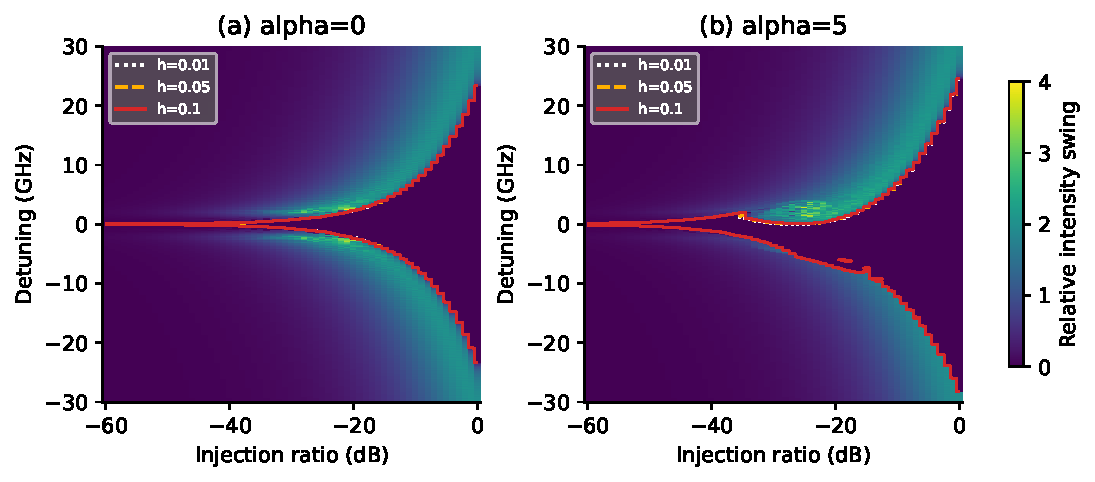
\includegraphics[width=\linewidth]{images/review_threshold.pdf}
\caption{\textcolor{red}{\textbf{Empirical cutoff comparison.} Intensity-swing maps for \textbf{a)} $\alpha=0$ and \textbf{b)} $\alpha=5$, with contours of the joint conditions $\Delta I/\bar I\le h$ and $\Delta\phi\le h~\mathrm{rad}$ at $h=0.01$, 0.05, and 0.10. Color represents the original relative intensity swing. The comparison assesses the descriptive contour, rather than proving dynamical stability.}}
\label{fig:review-threshold}
\end{figure}

\clearpage
\subsection{\textcolor{red}{Modulation-Depth Coverage}}
\textcolor{red}{The Fig.~5 data cover modulation depths from 1\% to 100\% in 1\% increments. Figure~\ref{fig:review-depth} explicitly includes the 1\%, 5\%, and 10\% traces alongside the representative larger depths displayed in the main text. These curves are extracted from the original stored frequency-response arrays.}
\begin{figure}[htbp]
\centering
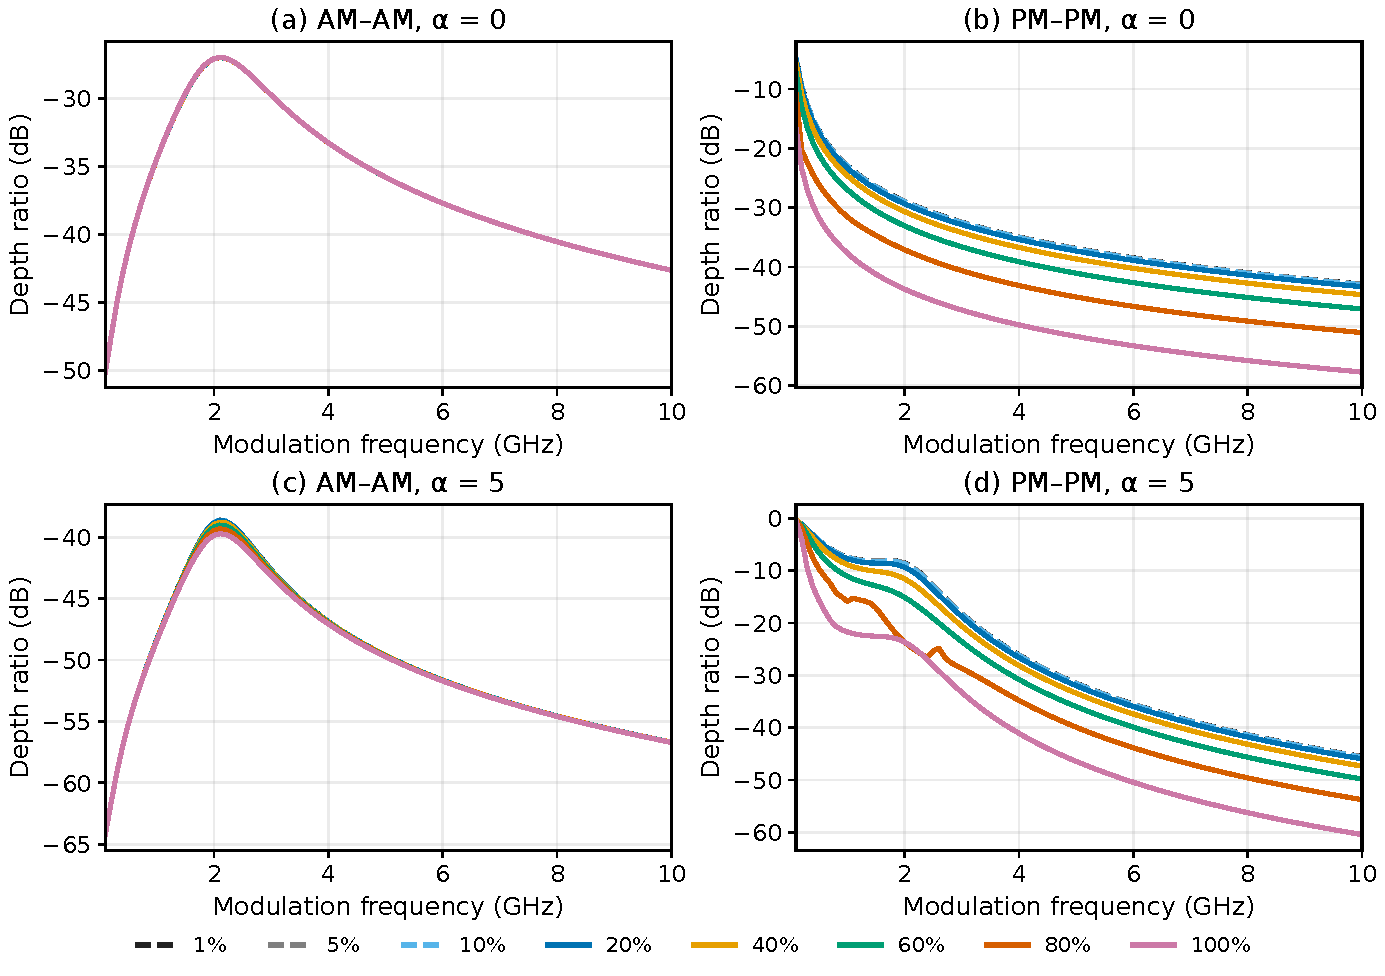
\includegraphics[width=\linewidth,height=0.60\textheight,keepaspectratio]{images/review_depth.pdf}
\caption{\textcolor{red}{\textbf{Expanded depth selection from the Fig.~5 sweeps.} AM$\to$AM and PM$\to$PM fundamental responses at $R_{\mathrm{inj}}=-50$~dB and zero detuning for \textbf{a,b)} $\alpha=0$ and \textbf{c,d)} $\alpha=5$. The displayed depths are 1\%, 5\%, 10\%, 20\%, 40\%, 60\%, 80\%, and 100\%; the underlying grid contains every 1\% increment.}}
\label{fig:review-depth}
\end{figure}

\clearpage
\subsection{\textcolor{red}{Complex-Field Readout and Facet Reflection}}
\textcolor{red}{For the additional computational assessment, the field incident on the local remodulator is modeled as
\[
E_{\mathrm{out}}(t)=E_s(t)+\sqrt{R_f}e^{i\theta_r}E_{\mathrm{inj}}(t),
\qquad E_B(t)=\frac{E_{\mathrm{out}}(t)}{C}\,y(t),
\]
where $E_s$ retains the residual amplitude and phase modulation from the rate equations. $R_f$ is a power reflectivity, so $R_f=0.30$ corresponds to a field coefficient $\sqrt{0.30}$ rather than 0.30. Both fields are expressed in the same effective output-plane units, with the intracavity-to-output conversion factor set to unity. This additive output model holds the laser parameters fixed; a device-specific treatment would also require facet coupling and output conversion to be calibrated.}

\textcolor{red}{The injection field is $A_{\mathrm{fr}}10^{R_{\mathrm{inj,dB}}/20}[1+x(t)]$. As in the symbol readout model, the data arm is the signed field $E_A=x(t)$, implying carrier-suppressed encoding in that arm. The differential signal is $2\operatorname{Re}\{E_AE_B^*\}$. The scalar $C$ is the mean complex no-reflection carrier over the final 10--1~ns before data onset and is shared by the reflection and no-reflection cases. It is not fitted to the data. Figure~\ref{fig:review-reflection} additionally distinguishes this fixed calibration from recalibration of the reflected CW output.}

\begin{figure}[htbp]
\centering
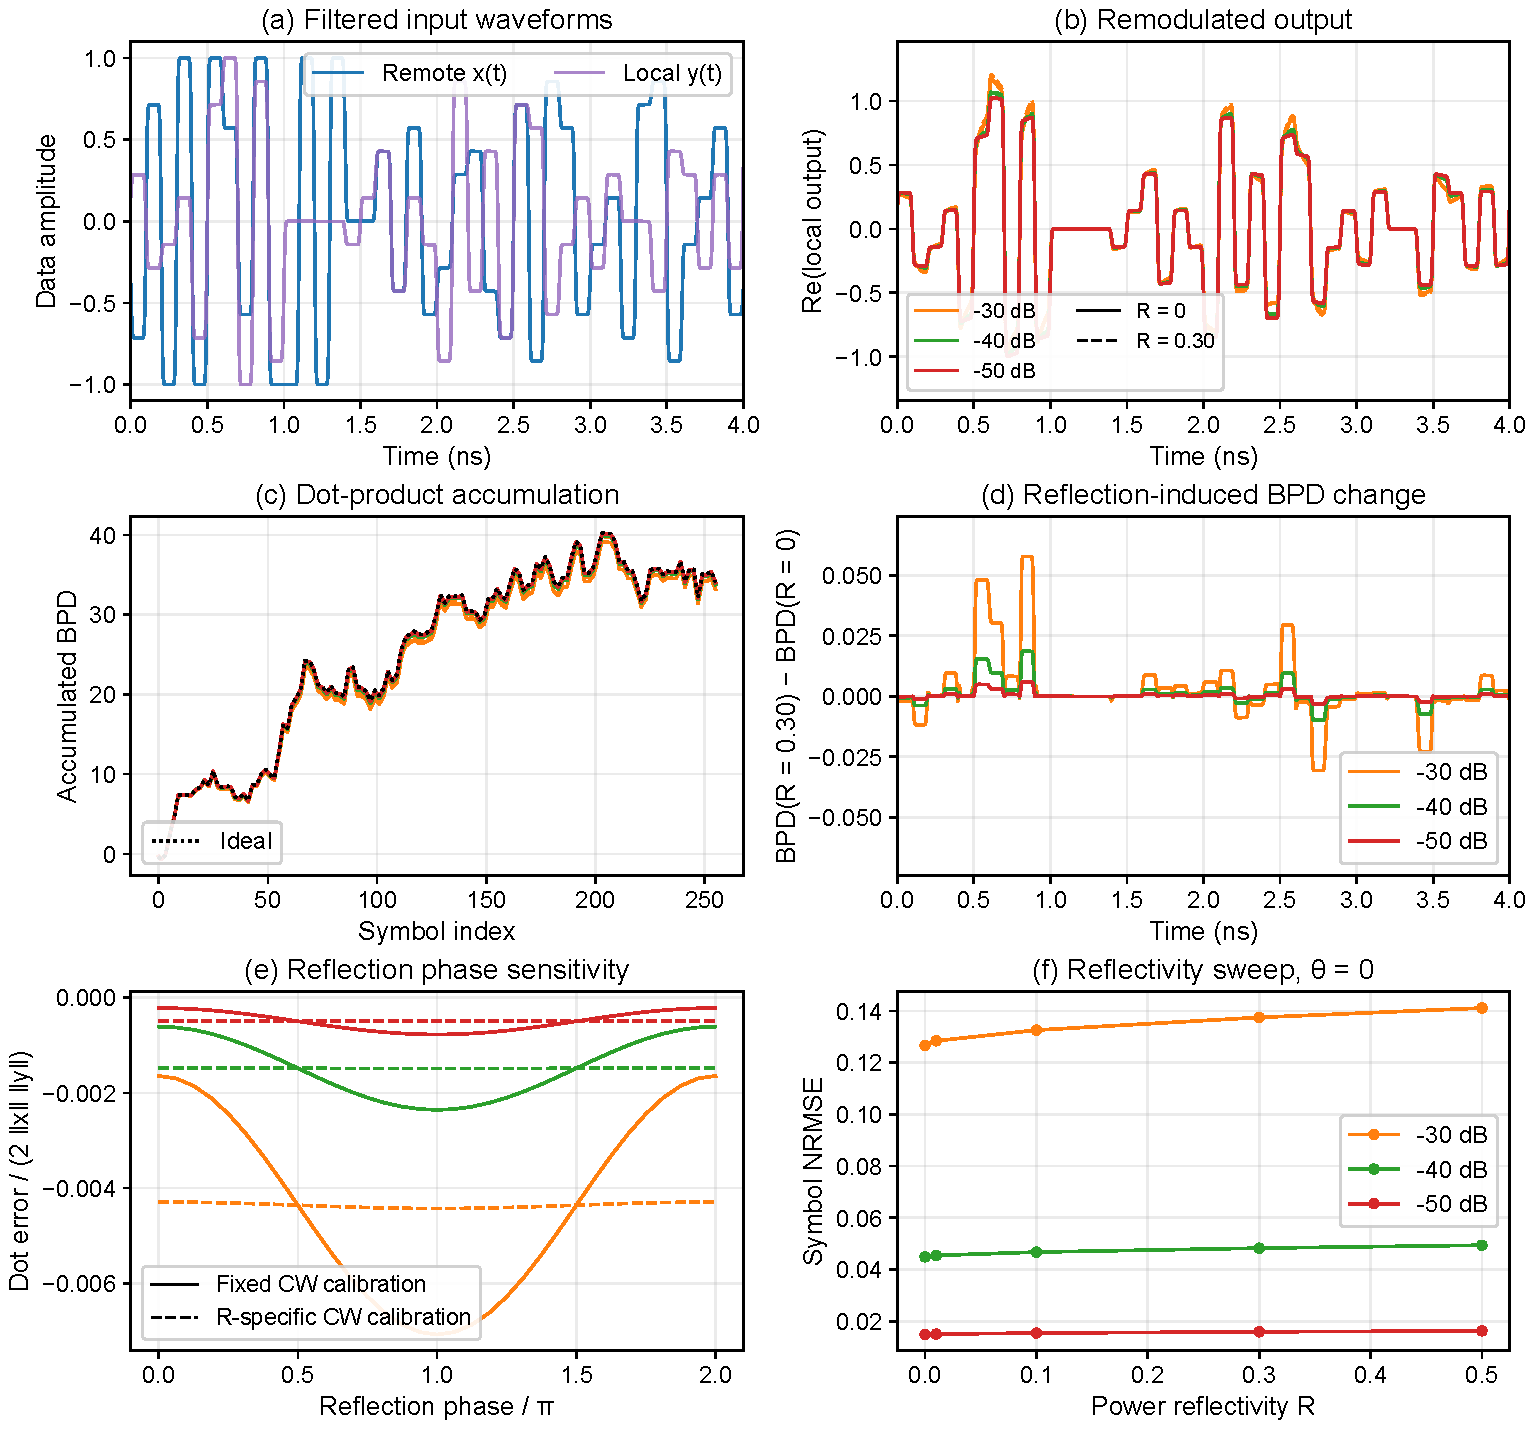
\includegraphics[width=\linewidth,height=0.57\textheight,keepaspectratio]{images/review_reflection.pdf}
\caption{\textcolor{red}{\textbf{Output reflection before local remodulation.} Example at $\alpha=0$, 10~Gbaud, and 256 encoded symbols. \textbf{a)} Filtered remote and local data. \textbf{b)} Locally remodulated field with $R_f=0$ and 0.30. \textbf{c)} Running dot product. \textbf{d)} Reflection-induced change in the differential signal. \textbf{e)} Reflection-phase dependence at $R_f=0.30$, with fixed and reflection-specific CW calibration. \textbf{f)} Symbol-error dependence on power reflectivity at $\theta_r=0$. Reflection can add to or partially cancel an existing error; one phase or sequence does not characterize its worst-case effect.}}
\label{fig:review-reflection}
\end{figure}

\clearpage
\subsection{\textcolor{red}{Ensemble Accuracy and Numerical Resolution}}
\textcolor{red}{Each sequence contains random signed magnitudes from eight equally spaced levels between zero and one, arranged in antipodal pairs. We use 32 independent sequence pairs for each encoded length $L=64$, 256, 1024, and 4096, with identical inputs across injection and reflection conditions. The Gaussian FIR cutoff is 20~GHz, with 64 samples per 10~Gbaud symbol. A 50~ns unmodulated interval precedes the data. The RK4 substep is 0.390625~ps; halving it changes the symbol outputs by at most $1.3\times10^{-8}$ in relative norm for the checked $\alpha=0,5$ and $-30,-50$~dB cases.}

\textcolor{red}{The reference $z_q^{\mathrm{id}}$ is obtained by integrating $2x(t)y(t)$ with the same filtering and symbol windows. For sequence $q$, let $e_q=z_q-z_q^{\mathrm{id}}$. We report
\[
\mathrm{RMSE}=\sqrt{\frac{1}{Q}\sum_q e_q^2},\qquad
\mathrm{NRMSE}=\sqrt{\frac{\sum_q e_q^2}{\sum_q(z_q^{\mathrm{id}})^2}},
\]
the Pearson correlation across sequences, and $|e_q|/(2\|\mathbf{x}_q\|_2\|\mathbf{y}_q\|_2)$ using the unfiltered symbol vectors in the last denominator. This avoids division by an individual dot product near zero. Confidence intervals use 2000 bootstrap resamples. These are deterministic model comparisons; no detector shot noise or experimentally calibrated laser noise is included.}

\begin{figure}[htbp]
\centering
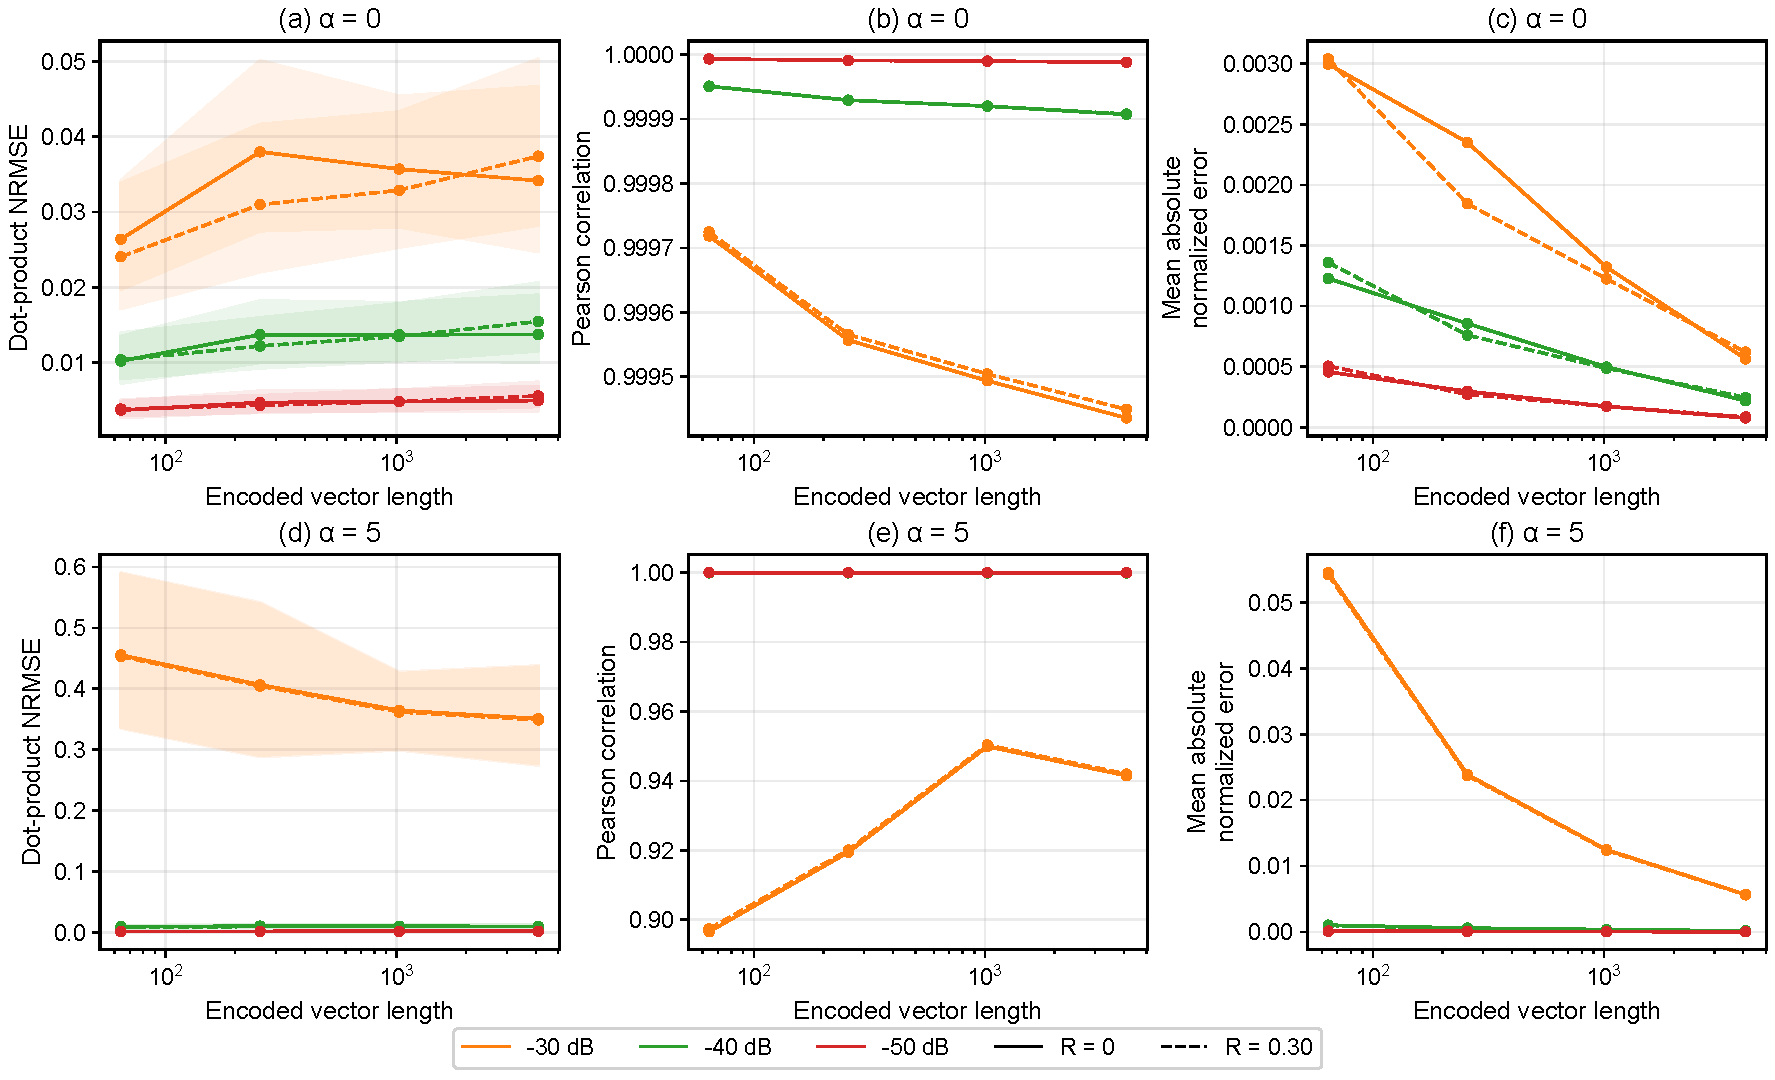
\includegraphics[width=\linewidth,height=0.54\textheight,keepaspectratio]{images/review_ensemble.pdf}
\caption{\textcolor{red}{\textbf{Additional ensemble metrics.} Rows correspond to $\alpha=0$ and 5. Columns show NRMSE, Pearson correlation, and mean absolute norm-normalized error versus encoded vector length, for 32 independent sequence pairs per length. Solid curves omit reflection and dashed curves use $R_f=0.30$, $\theta_r=0$. Shaded NRMSE bands indicate bootstrap 95\% confidence intervals. The main-text Fig.~7 shows the compact NRMSE comparison.}}
\label{fig:review-ensemble}
\end{figure}

\clearpage
\subsection{\textcolor{red}{Common Phase and Frequency-Drift Scenarios}}
\textcolor{red}{To illustrate the distinction between static detuning tolerance and dynamic phase tracking, we apply a common input phase modulation of amplitude 0.3~rad at 1, 10, and 100~MHz with $\alpha=0$. Figure~\ref{fig:review-phase} shows the phase difference between the recovered carrier and the received field, evaluated after transients. These prescribed perturbations are sensitivity tests, rather than measured acoustic or thermal fiber-noise spectra.}

\textcolor{red}{A separate test applies sinusoidal relative-frequency drift with 100~MHz amplitude at 1~MHz. We compare the uncompensated detuning $d(t)$ with $d(t)-\hat d(t)$, where $50~\mathrm{ns}\,d\hat d/dt+\hat d=d$. This idealized first-order correction assumes access to the detuning and illustrates the benefit of maintaining the laser within the operating interval; it does not simulate an experimental error detector or temperature-control loop.}
\begin{figure}[htbp]
\centering
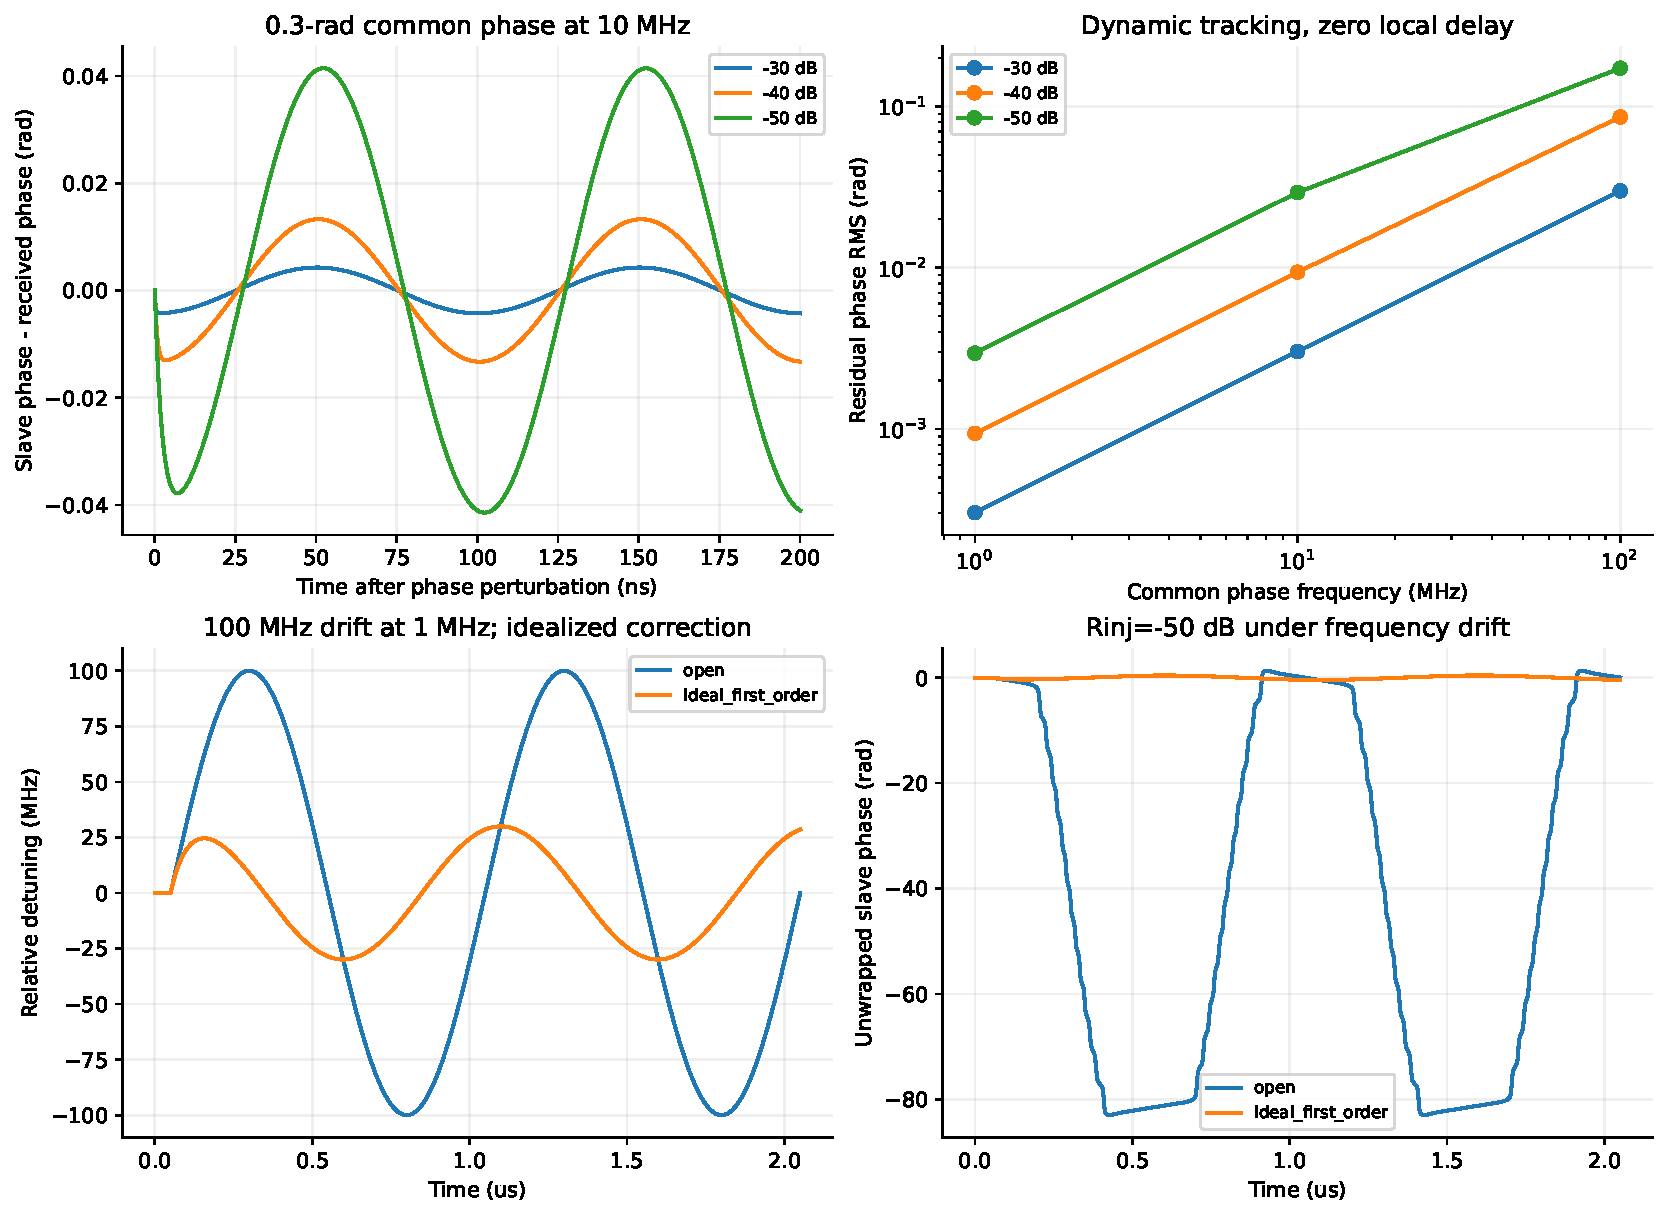
\includegraphics[width=\linewidth,height=0.58\textheight,keepaspectratio]{images/review_phase.pdf}
\caption{\textcolor{red}{\textbf{Dynamic phase and detuning response.} Upper left: residual phase under 0.3-rad common phase modulation at 10~MHz. Upper right: residual RMS phase versus modulation frequency for three injection ratios, with zero differential path delay. Lower left: imposed detuning before and after idealized first-order correction. Lower right: the corresponding unwrapped injected-laser phase at $R_{\mathrm{inj}}=-50$~dB. The calculation illustrates phase-tracking and drift sensitivity under specified deterministic perturbations.}}
\label{fig:review-phase}
\end{figure}
\clearpage
% REVIEW-ADD-END supplementary results

\bibliography{refs}

\end{document}
